\section{Background: Distributed Databases \& Big Data}\label{sec:distributed}

\subsection{Introduction}
We ask: does the world have any precedents for \textit{distributed databases} at massive scale? The answer is yes.
All large Internet companies, and many small ones, run “big data” distributed databases (DBs), including Facebook, Google, Amazon and Netflix.

Distributed DBs regularly store petabytes ($1,000,000$ GB) or more worth of content. 
In contrast, the Bitcoin blockchain currently stores $50$ GB, the capacity of a modern thumb drive.
Despite it's relatively-small data size, members of the Bitcoin community worry that it is getting too big. In fact, there are initiatives to prevent “blockchain bloat” caused by “dust” or “junk” transactions that “pollute” Bitcoin’s $50$ GB database \cite{wagner2014blockchain_bloat}.

Let’s look at it another way: perhaps distributed DB technology has lessons for blockchain DB design.

\medskip
\centerline{Let’s explore distributed DB scalability further.}

\begin{figure}[!ht]
  \centering
  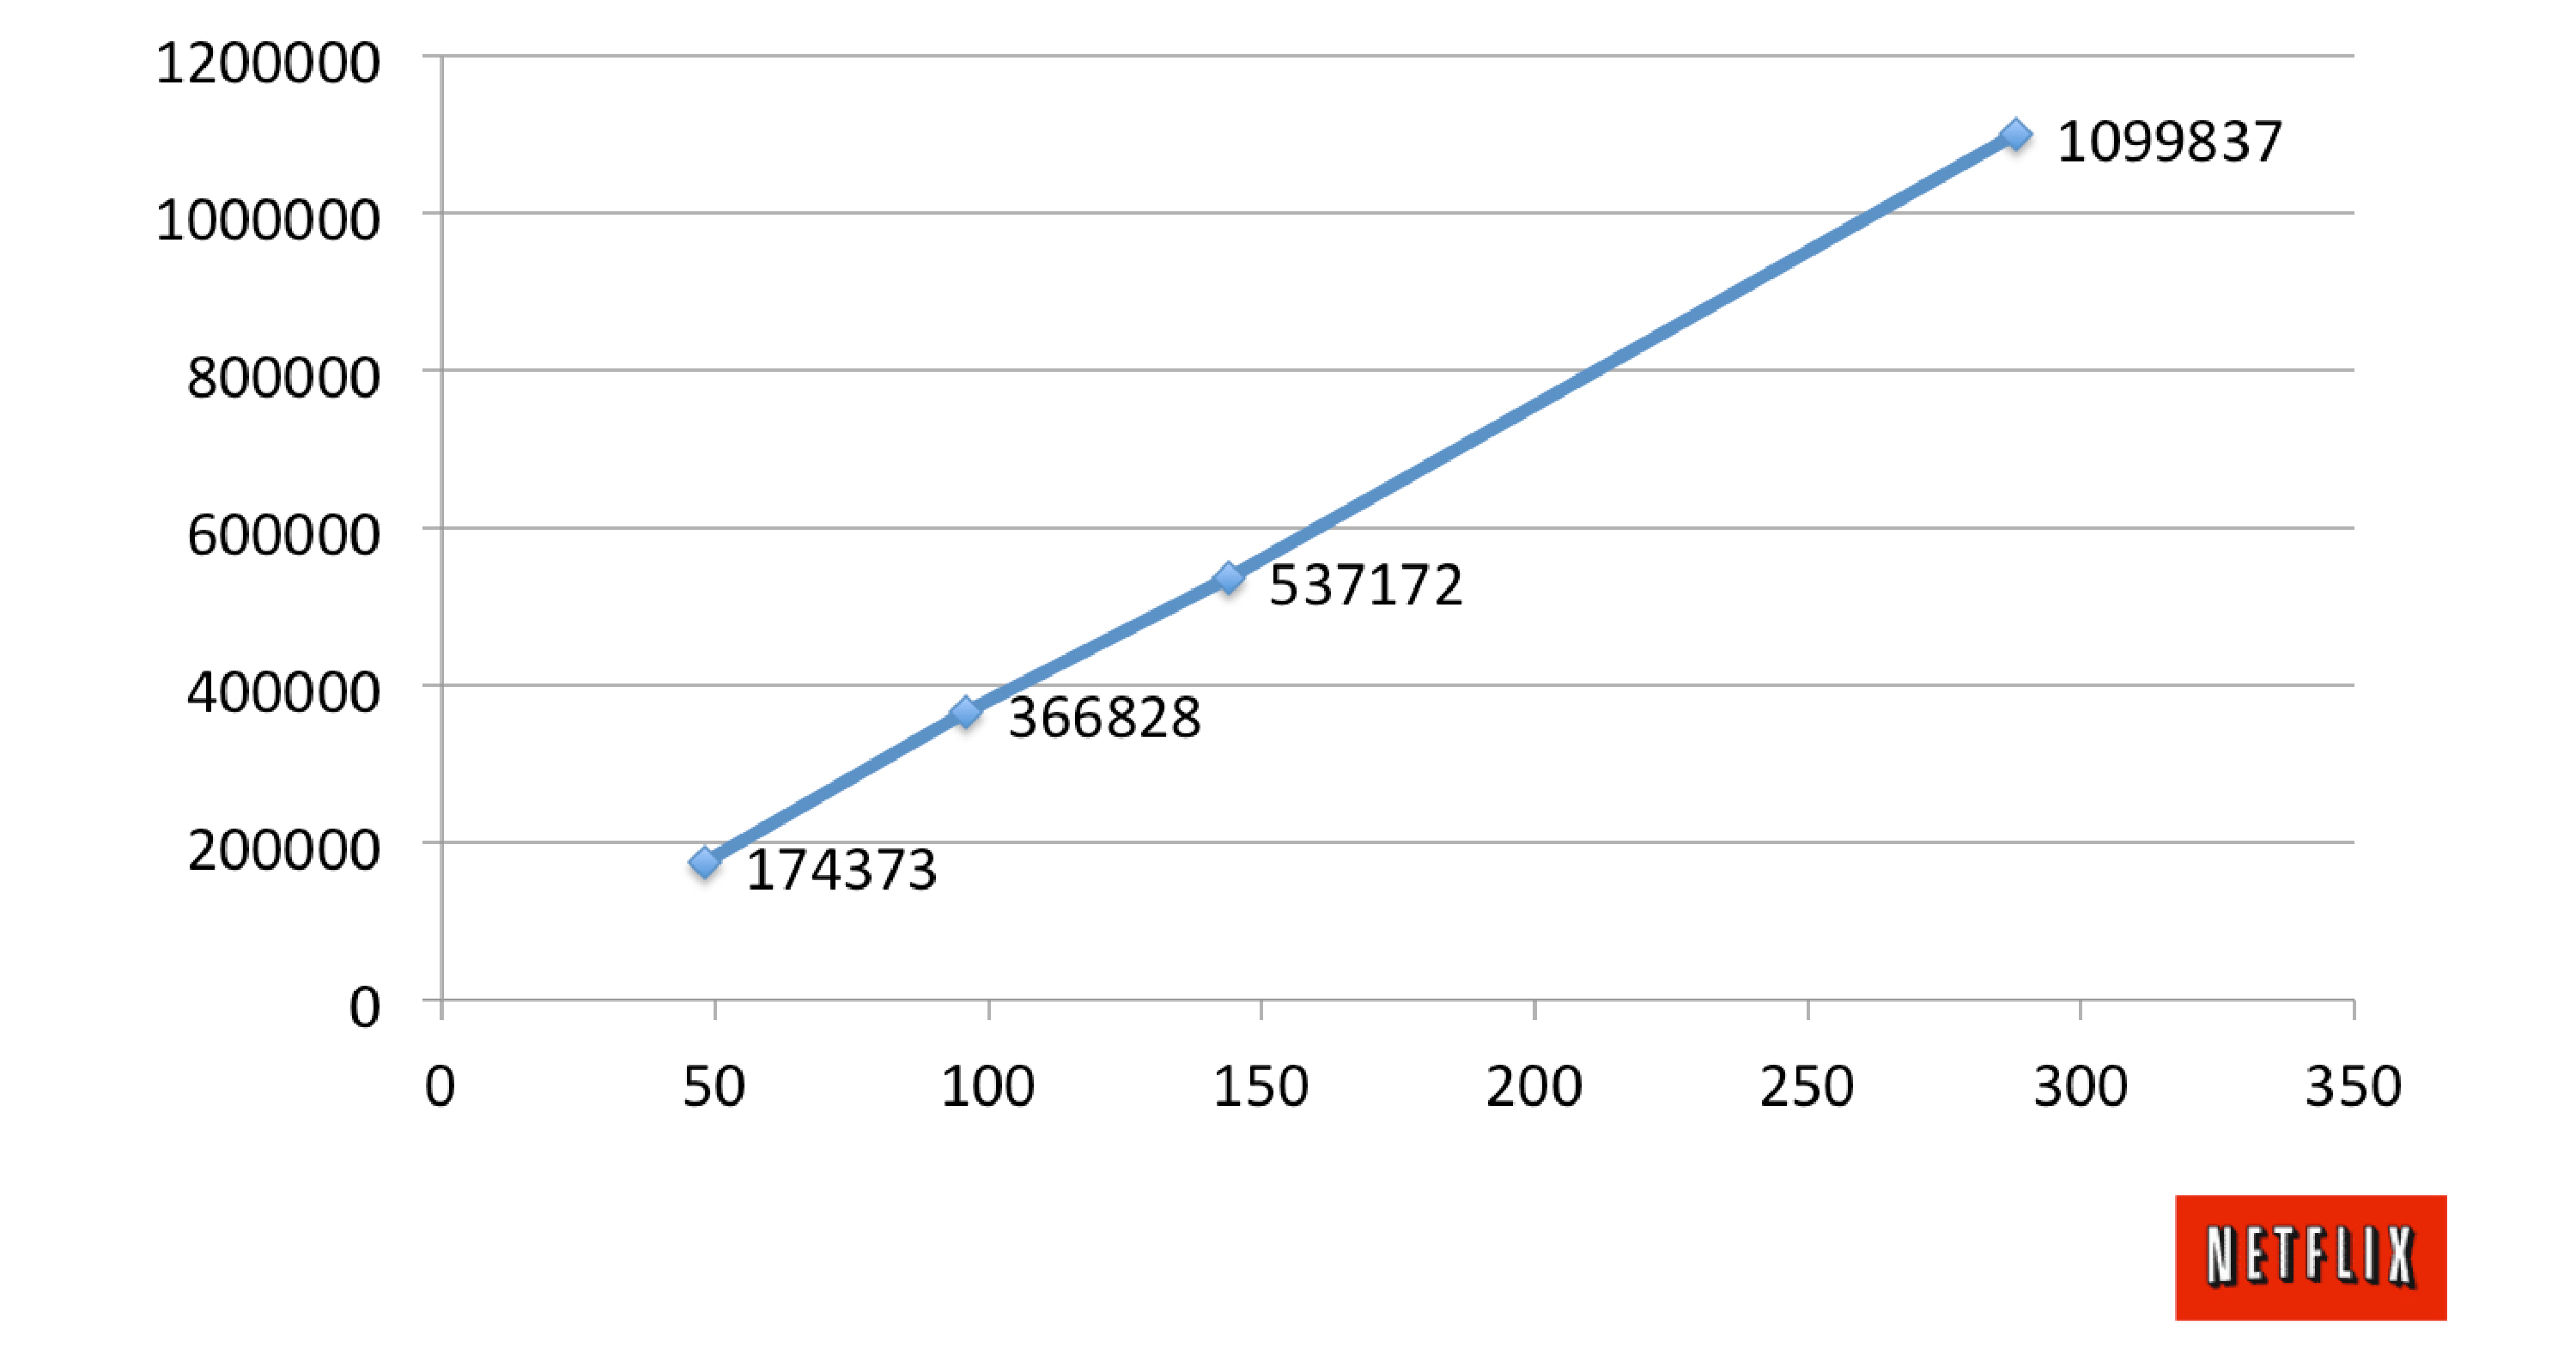
\includegraphics[width=\textwidth]{figure_2.pdf}
  \caption{Netflix experimental data on throughput of its Cassandra database (Client writes/s by node count - Replication Factor=$3$).
  The x-axis is number of nodes; the y-axis is writes per second. From \cite{cockcroft2011benchmarking}.}
  \label{fig:cassandra_throughput}
\end{figure}

\medskip
Figure \ref{fig:cassandra_throughput} illustrates the throughput properties of Cassandra, a distributed DB technology used by Netflix.
At the bottom left of the plot, we see that $50$ distributed Cassandra nodes could handle $174,000$ writes per second.
Increasing to $300$ nodes allowed for $1.1$ million writes per second \cite{cockcroft2011benchmarking}.
A follow-up study three years later showed a throughput of $1$ million writes per second with just a few dozen nodes \cite{kalantzis_netflix}.
To emphasize: the throughput of this DB increased as the number of nodes increased. The scaling is linear: $10\times$ more nodes means $(10c)\times$ more throughput, where $0 < c \leq 1$.

Each node also stores data.
Critically, a node only stores a subset of all data, that is, it has partial replication.
In the Netflix example \cite{kalantzis_netflix}, each piece of data has three copies in the system, i.e. a replication factor of three.
Partial replication enables an increase in the number of nodes to increase storage capacity.
Most modern distributed DBs have a linear increase in capacity with the number of nodes, an excellent property.
Additionally, as the number of nodes increases, Cassandra’s latency and network usage does not worsen.
Cassandra can be distributed at scale not only throughout a region, but around the globe.
Contrast this to the Bitcoin blockchain, where capacity does not change as the number of nodes increases.

The scalability properties of distributed DBs like Cassandra make an excellent reference target.

\subsection{Consensus Algorithms in Distributed Databases}\label{subsec:consensus}
\subsubsection{Introduction}
As mentioned above, Cassandra keeps only some of the data in each node. Each bit of data is replicated on several nodes. The nodes responsible for replicating a bit of data use a consensus algorithm to ensure they agree on what to store. Cassandra uses the Paxos consensus algorithm; the relevant nodes will reach agreement even if some of them are unresponsive.

The Paxos consensus algorithm is one of many algorithms designed to solve the \emph{consensus problem} in unreliable distributed systems. Loosely speaking, the consensus problem is the problem of figuring out how to get a bunch of isolated computing processes to agree on something, when some of them may be faulty, and they can only communicate by two-party messages. A solution takes the form of a consensus algorithm/protocol used by all of the non-faulty processes.

\subsubsection{Byzantine Fault Tolerance}
One of the first precise statements of the consensus problem was in a 1980 paper by Pease, Shostak and Lamport \cite{pease1980reaching,lamport_writings}. That paper allowed the faulty processes to have arbitrary faults; for example, they could lie, collude, selectively participate, or pretend to be crashed. Such arbitrary faults are also known as \emph{Byzantine faults}, after a 1982 follow-up paper on the same problem \cite{lamport1982byzantine} which called it the ``Byzantine Generals Problem.'' A consensus algorithm which enables a distributed system to come to consensus despite Byzantine faults is said to be \emph{Byzantine fault tolerant} (BFT).

The 1980 paper had several nice results:
a proof that, given $f$ Byzantine faulty processes, at least $3f+1$ processes are needed,
an example (inefficient) solution with $3f+1$ processes, 
and a proof that there is \emph{no} solution with less than $3f+1$ processes.
It also considered what's possible if message authentication is used (i.e. if a process changes a message before relaying it to another process, then the change can be detected). In that case, $2f+1$ processes suffice.

\subsubsection{(Benign) Fault Tolerance}
One of the most common ways for a process to be faulty is for it to be unresponsive. That can happen, for example, if a hard drive fails or a CPU overheats. Such faults are known as \emph{benign faults} or \emph{fail-stop faults}. A consensus algorithm which enables a distributed system to come to consensus despite benign faults is said to be \emph{fault tolerant} (FT). (It would be more precise to say ``benign-fault tolerant,'' but it's not up to us.) In general, fault-tolerant consensus algorithms require at least $2f+1$ processes to be able to tolerate up to $f$ faulty processes.

\subsubsection{Paxos}
The best-known fault-tolerant consensus algorithm is Paxos; it was first published by Lamport in 1998 \cite{lamport1998part}. Since then, many variations have been developed (e.g. ``Fast Paxos'' \cite{lamport2006fast}) so there is now a whole family of Paxos algorithms, including some that are BFT. \cite{lamport2011byzantizing}

Mike Burrows of Google (co-inventor of Google’s Chubby, BigTable, and Dapper) has said, ``There is only one consensus protocol, and that’s Paxos,'' \cite{robinson2009paxos} and ``all working protocols for asynchronous consensus we have so far encountered have Paxos at their core.'' \cite{burrows2006chubby}
Henry Robinson of Cloudera has said, ``all other approaches are just broken versions of Paxos'' and ``it’s clear that a good consensus protocol is surprisingly hard to find.'' \cite{robinson2009paxos}

Paxos and its lineage are used at Google, IBM, Microsoft, OpenReplica, VMWare, XtreemFS, Heroku, Ceph, Clustrix, Neo4j, and many more. \cite{wiki_paxos}

Paxos is notoriously difficult to understand and risky to implement.
To address this, Raft \cite{ongaro2014raft} was designed specifically for ease of understanding, and therefore has lower implementation risk.
Raft has a BFT variant named Tangaroa. \cite{copeland2014tangaroa}

\subsubsection{The FLP Result}
An \emph{asynchronous process} is a process which can't promise it will get back to you with a result within some time limit. It's common to model processes as being asynchronous, especially for large systems spread all over the globe (such as the World Wide Web). An \emph{asynchronous consensus protocol} is one that works with asynchronous processes.

In 1985, Fischer, Lynch and Paterson (FLP) published a surprising result: ``no completely asynchronous consensus protocol can tolerate even a single unannounced process death [i.e. benign fault].'' \cite{fischer1985impossibility} If that's the case, then it seems there's little hope for tolerating more faults (or other kinds of faults)! Practical consensus algorithms can get around the ``FLP result'' by assuming some kind of synchrony (e.g. ``partial synchrony'' or ``weak synchrony''), or by allowing some form of probablistic consensus (e.g. with the probability of consensus approaching 1 over time).

Bitcoin's consensus algorithm does the latter: one can never be sure that the Bitcoin network has come to consensus about a block being in the final blockchain: there's always the possibility that block might be in a side branch. All one can do is estimate the probability that a block is in the final blockchain.

\subsubsection{Practical BFT Consensus Algorithms}
The early BFT consensus algorithms were either slow \& expensive, or intended for synchronous systems \cite{wiki_byzantine,paulitsch2005coverage,hopkins1987evolution,driscoll1983multi}. That all changed in 1999, when Castro and Liskov published their paper titled ``Practical Byzantine Fault Tolerance'' (PBFT) \cite{castro1999practical,castro2001byzantine}. As the title suggests, it described a more practical (usable) BFT consensus algorithm, and kicked off a flurry of research into practical BFT consensus algorithms.
That research continues today. Aardvark \cite{clement2009making}, RBFT \cite{aublin2013rbft} and Stellar \cite{mazieres2015stellar} are examples of algorithms aimed at improving speed and reliability.


\subsection{Replication Factor \& Blockchain “Full Nodes”}
A modern distributed DB is designed to appear like a single monolithic DB, but under the hood it distributes storage across a network holding many cheap storage devices.
Each data record is stored redundantly on multiple drives, so if a drive fails the data can still be easily recovered.
If only one disk fails at a time, there only needs to be one backup drive for that data.
The risk can be made arbitrarily small, based on assumptions of how many disks might fail at once.
Modern distributed DBs typically have three backups per data object, i.e. a replication factor of $3$ \cite{wiki_raid}.

In contrast, Bitcoin has about $6,500$ full nodes \cite{bitcoin2015fees}—a replication factor of $6,500$.
The chance of all nodes going down at once in any given hour (assuming complete independence) is $(1/8760)^{6500}$, or $10^{-25626}$.
The chance of all nodes going down would occur once every $3,000$ billion years. To say this is overkill is to put it mildly.

Of course, hardware failure is not the only reason for lost data.
Attacks against the nodes of the network have a much higher probability of destroying data.
A well-targeted attack to two or three mining pools could remove $50\%$ of the computing power from the current Bitcoin network, making the network unusable until the next adjustment to POW complexity, which happens about every two weeks.

\subsection{Strengths and Weaknesses}
Let’s review the strengths and weaknesses of DBs that use distributed consensus algorithms such as Paxos.

\medskip
\noindent\textbf{Strengths.} As discussed above, Paxos is a field-proven consensus algorithm that tolerates benign faults (and extensions for Byzantine tolerance have been developed).
It is used by “big data” distributed DBs with the well-documented ability to handle high throughput, low latency, high capacity, efficient network utilization, and any shape of data, including table-like SQL interfaces, object structures of NoSQL DBs, and graph DBs, and they handle replication in a sane fashion.
Raft, a Paxos derivative, makes distributed consensus systems easier to design and deploy.

\medskip
\noindent\textbf{Weaknesses.} While their technical attributes and performance are impressive, traditional “big data” distributed DBs are not perfect: they are centralized.
They are deployed by a single authority with central control, rather than decentralized control as in blockchains.
This creates a number of failings.
Centralized DBs are:
\begin{itemize}
  \item \textbf{Controlled by a single admin user} so that if the admin user (or account) gets compromised, then the entire database might become compromised.
  \item \textbf{Mutable.} A hacker could change a 5-year-old record without anyone noticing (assuming no additional safeguards in place). For example, this would have prevented police from doctoring evidence in the India exam scandal \cite{sethy2015india_scam}. In blockchains, tampering with past transactons usually quite difficult. Even if someone does manage to change a past transaction, the change is easy to spot, because the hash of its block get stored in the next block; an auditor would detect a hash mismatch.
  \item \textbf{Not usable by participants with divergent interests} in situations where they do not want to cede control to a single administrator. For example, the risk of losing control of the management of information is one reason that copyright rightsholders in the music industry do not share a single DB.
  \item \textbf{Not designed to stop Sybil attacks}, where one errant node can swamp all the votes in the system.
  \item \textbf{Traditionally without support for the creation and transfer of digital assets} where only the owner of the digital asset, not the administrator of the DB, can transfer the asset.
  \item \textbf{Not typically open to the public} to read, let alone write. Public openness is important for public utilities. A notable exception is Wikidata \cite{wikidata}.
\end{itemize}

\subsection{Fault Tolerance in the BigchainDB System}

Simultaneously preserving the scalability and trustless decentralization of both large-scale databases and decentralized blockchains is the main objective of the BigchainDB system. The following were considered when designing BigchainDB's security measures:

\begin{itemize}
  \item \textbf{Benign faults}: In the BigchainDB setup, nodes communicate through a database which uses a fault-tolerant consensus protocol such as Raft or Paxos. Hence we can assume that if there are $2f + 1$ nodes, $f$ benign-faulty nodes can be tolerated (at any point in time) and each node sees the same order of writes to the database.
  \item \textbf{Byzantine faults}: In order to operate in a trustless network, BigchainDB incorporates measures against malicious or unpredictable behavior of nodes in the system. These include mechanisms for voting upon transaction and block validation. Efforts to achieve full Byzantine tolerance are on the roadmap and will be tested with regular security audits.
  \item \textbf{Sybil Attack}: Deploying BigchainDB in a federation with a high barrier of entry based on trust and reputation discourages the participants from performing an attack of the clones. The DNS system, for example, is living proof of an Internet-scale distributed federation. Appendix \ref{sec:dns} describes how the DNS has successfully run a decentralized Internet-scale database for decades.
\end{itemize}